\chapter{จุลินทรีย์ส่งเสริมการเจริญเติบโตของพืช (PGPR) และไมคอร์ไรซา}
\label{ch:pgpr}

\begin{keyconcept}[แนวคิดสำคัญของบทที่ 3]
แบคทีเรียบริเวณไรโซสเฟียร์ที่ส่งเสริมการเจริญเติบโตของพืช (Plant Growth-Promoting Rhizobacteria: PGPR) และเชื้อราไมคอร์ไรซา (Mycorrhizal Fungi) เป็นหัวใจสำคัญของเทคโนโลยีชีวภาพการเกษตรยุคใหม่ จุลินทรีย์กลุ่มนี้มีปฏิสัมพันธ์เชิงบวกกับระบบรากพืชผ่านกลไกที่หลากหลาย ทั้งการส่งเสริมการเติบโตโดยตรง (Direct Mechanisms) เช่น การสังเคราะห์ฮอร์โมนออกซิน การลดฮอร์โมนเอทิลีนสภาวะเครียดด้วยเอนไซม์ ACC Deaminase การตรึงไนโตรเจน และการละลายแร่ธาตุ และกลไกส่งเสริมโดยอ้อม (Indirect Mechanisms) เช่น การแย่งชิงไอออนเหล็กด้วยไซเดอโรฟอร์ และการชักนำระบบภูมิคุ้มกันความต้านทานโรคทั้งระบบของพืช (Induced Systemic Resistance: ISR) การทำความเข้าใจกลไกระดับโมเลกุลช่วยให้นักวิจัยสามารถคัดเลือกและผสมผสานสายพันธุ์จุลินทรีย์เป็นสูตรหัวเชื้อร่วม (Microbial Consortia) ที่มีประสิทธิภาพสูงในแปลงเกษตรจริง
\end{keyconcept}

\begin{figure}[ht]
    \centering
    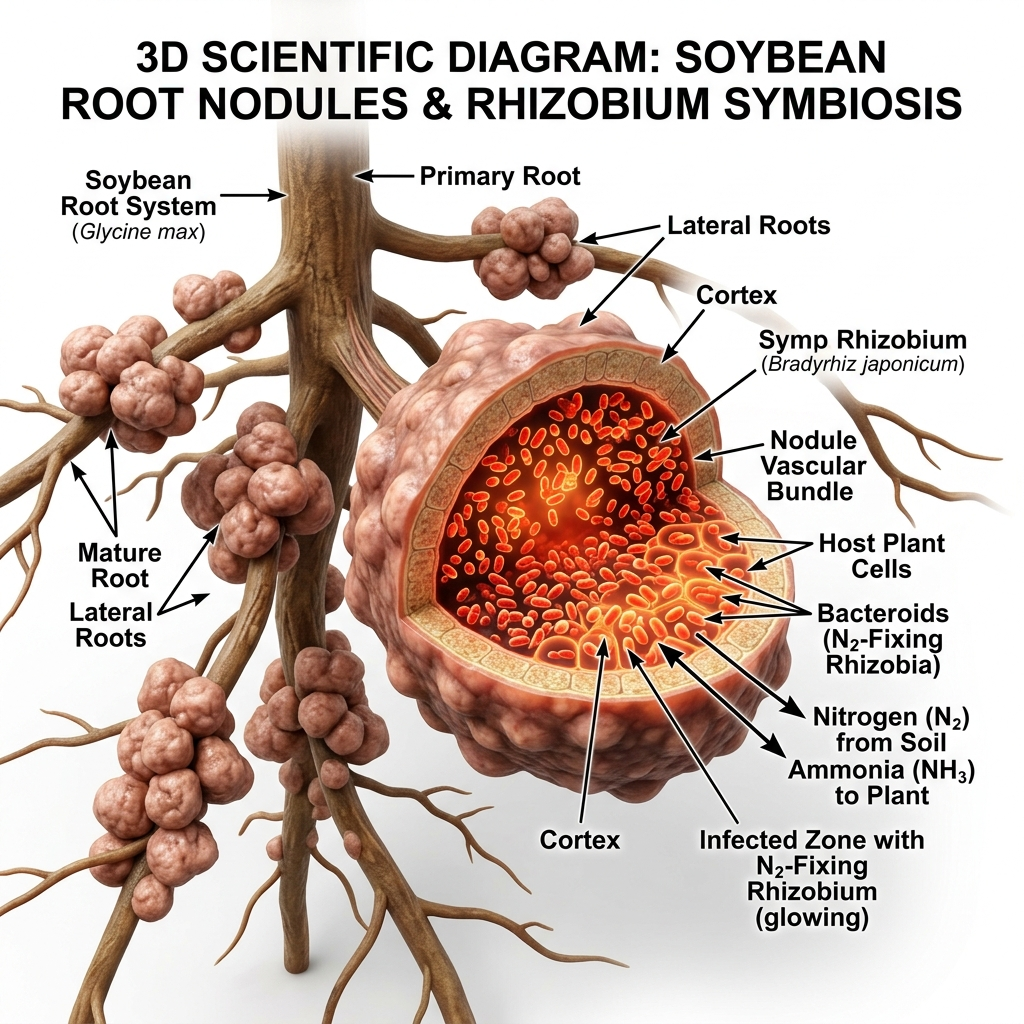
\includegraphics[width=0.85\textwidth]{assets/ch03_root_nodules.png}
    \caption{โครงสร้าง 3D ตัดขวางของปมรากพืชตระกูลถั่ว แสดงท่อติดเชื้อ (Infection thread) และกลุ่มเซลล์แบคทีรอยด์ (Bacteroids) ของเชื้อ \organism{Rhizobium} ด้านในเซลล์พืชที่ถูกห่อหุ้มในซิมไบโอโซม (Symbiosome) ล้อมรอบด้วยโปรตีนเลกเฮโมโกลบินสีแดง}
    \label{fig:ch03_root_nodules}
\end{figure}

\section*{วัตถุประสงค์การเรียนรู้ประจำบท}
เมื่อศึกษาบทเรียนนี้จบแล้ว นักศึกษาสามารถ:
\begin{enumerate}
    \item อธิบายความหมาย การจำแนกประเภท และความแตกต่างระหว่าง ePGPR และ iPGPR
    \item วิเคราะห์วิถีชีวเคมีของการสังเคราะห์ฮอร์โมนพืช (IAA) และกลไกการลดความเครียดพืชด้วยเอนไซม์ ACC Deaminase
    \item เปรียบเทียบความแตกต่างระหว่างระบบภูมิคุ้มกันพืช ISR (ชักนำโดย PGPR) และ SAR (ชักนำโดยเชื้อก่อโรค)
    \item อธิบายลำดับขั้นตอนโมเลกุลการส่งสัญญาณ Nod Factors ระหว่างพืชตระกูลถั่วกับ \organism{Rhizobium}
    \item วิเคราะห์บทบาทของเชื้อราอาร์บัสคูลาร์ไมคอร์ไรซา (AMF) ต่อการดูดซึมฟอสฟอรัสและการสร้างสารกลอมาลินในดิน
\end{enumerate}

\section{นิยามและการจัดจำแนกกลุ่ม PGPR}

คำว่า \textbf{PGPR (Plant Growth-Promoting Rhizobacteria)}\index{PGPR (Plant Growth-Promoting Rhizobacteria)} ถูกบัญญัติขึ้นครั้งแรกโดย Joseph W. Kloepper และ Milton N. Schroth ในปี ค.ศ. 1978 เพื่ออธิบายกลุ่มแบคทีเรียดินที่อาศัยอยู่หนาแน่นบริเวณรอบรากพืชและมีผลในการกระตุ้นการเจริญเติบโตของพืชอย่างชัดเจน จุลินทรีย์กลุ่มนี้จำแนกออกเป็น 2 กลุ่มใหญ่ตามความลึกของการอยู่อาศัยในเนื้อเยื่อพืช:

\begin{enumerate}
    \item \textbf{แบคทีเรียภายนอกเซลล์พืช (Extracellular PGPR: ePGPR):\index{ePGPR (Extracellular PGPR)}} ดำรงชีวิตอยู่บริเวณผิวสัมผัสราก (Rhizoplane) หรือในช่องว่างดินรอบราก (Rhizosphere) โดยไม่แทรกซึมเข้าไปในเนื้อเยื่อพืช ได้แก่ แบคทีเรียสกุล \organism{Pseudomonas}, \organism{Bacillus}, \organism{Azotobacter}, \organism{Azospirillum}, \organism{Serratia}, และ \organism{Streptomyces}
    \item \textbf{แบคทีเรียภายในเซลล์พืช (Intracellular PGPR: iPGPR):\index{iPGPR (Intracellular PGPR)}} สามารถแทรกซึมผ่านเซลล์ชั้นนอกเข้าไปอาศัยอยู่ภายในเซลล์เยื่อหุ้มของพืชอย่างจำเพาะเจาะจง โดยพืชจะสร้างอวัยวะพิเศษขึ้นมารองรับ ได้แก่ แบคทีเรียกลุ่มสร้างปมรากถั่วสกุล \organism{Rhizobium}, \organism{Bradyrhizobium}, \organism{Sinorhizobium}, และกลุ่มแอคติโนมัยซีสสร้างปมในพืชป่าสกุล \organism{Frankia}
\end{enumerate}

\section{กลไกส่งเสริมการเจริญเติบโตโดยตรง (Direct Mechanisms)}

\subsection{1. การสังเคราะห์ฮอร์โมนพืช (Phytohormone Biosynthesis)}

จุลินทรีย์ PGPR มากกว่าร้อยละ 80 มีความสามารถในการสังเคราะห์ฮอร์โมนพืชกลุ่มออกซิน โดยเฉพาะ \textbf{กรดอินโดล-3-อะซิติก (Indole-3-acetic acid: IAA)\index{กรดอินโดล-3-อะซิติก (IAA)}\index{Indole-3-acetic acid (IAA)}} ซึ่งแบคทีเรียใช้น้ำคั้นรากพืชที่มีกรดอะมิโนทริปโตเฟน (L-tryptophan) เป็นสารตั้งต้น ผ่าน 3 วิถีชีวเคมีหลัก:

\begin{itemize}
    \item \textbf{Indole-3-pyruvic acid (IPyA) Pathway:} เป็นวิถีหลักใน \organism{Pseudomonas} และ \organism{Azospirillum} โดยทริปโตเฟนถูกเปลี่ยนเป็น IPyA ด้วยเอนไซม์ Aminotransferase จากนั้นเปลี่ยนเป็น Indole-3-acetaldehyde (IAAld) และออกซิไดซ์เป็น IAA ในที่สุด
    \item \textbf{Indole-3-acetamide (IAM) Pathway:} พบเด่นชัดใน \organism{Agrobacterium} และ \organism{Pseudomonas syringae} ทริปโตเฟนถูกเปลี่ยนเป็น IAM ด้วยเอนไซม์ Tryptophan 2-monooxygenase และเปลี่ยนเป็น IAA ด้วยเอนไซม์ IAM hydrolase
    \item \textbf{Tryptamine (TAM) Pathway:} ทริปโตเฟนถูกเปลี่ยนเป็น Tryptamine ก่อนเปลี่ยนเป็น IAAld และ IAA
\end{itemize}

IAA ที่จุลินทรีย์หลั่งออกมาจะกระตุ้นการขยายตัวของเซลล์ราก (Cell Elongation) และส่งเสริมการแตกแขนงของรากฝอย (Lateral roots and root hairs) ซึ่งช่วยเพิ่มพื้นที่ผิวในการดูดซับน้ำและธาตุอาหารของพืชได้อย่างมหาศาล

\subsection{2. การลดความเครียดพืชด้วยเอนไซม์ ACC Deaminase}

เมื่อพืชประสบสภาวะเครียดจากสิ่งแวดล้อม เช่น ภัยแล้ง (Drought) ดินเค็ม (Salinity) หรือสารเคมีสะสม พืชจะสังเคราะห์ฮอร์โมนเอทิลีน (Ethylene) สูงขึ้นอย่างรวดเร็ว โดยผ่านสารตั้งต้นคือ \textbf{1-aminocyclopropane-1-carboxylic acid (ACC)} ฮอร์โมนเอทิลีนในระดับที่สูงเกินไป (Stress Ethylene)\index{เอทิลีนในสภาวะเครียด (Stress Ethylene)} จะสั่งการให้รากหยุดการยืดตัว ใบเหลือง และใบร่วงเฉับพลัน

\begin{equation}
\text{S-Adenosylmethionine (SAM)} \xrightarrow{\text{ACC Synthase}} \text{ACC} \xrightarrow{\text{ACC Oxidase}} \text{Ethylene}
\end{equation}

แบคทีเรีย PGPR ที่มีเอนไซม์ \textbf{ACC Deaminase\index{ACC Deaminase}} (เช่น \organism{Pseudomonas putida} สายพันธุ์ UW4) จะเข้าจับและสลายสาร ACC ที่รากพืชหลั่งออกมาให้แตกตัวเป็นสารที่ไม่เป็นพิษ:

\begin{equation}
\text{ACC} + H_2O \xrightarrow{\text{ACC Deaminase}} \alpha\text{-ketobutyrate} + NH_3
\end{equation}

แบคทีเรียจะนำแอมโมเนียและแอลฟา-คีโตบิวไทเรตไปใช้เป็นแหล่งไนโตรเจนและพลังงาน ส่งผลให้ความเข้มข้นของ ACC บริเวณรากลดลง เกิดแรงขับดันให้พืชส่ง ACC ออกมาสู่ภายนอกอย่างต่อเนื่อง ระดับเอทิลีนในพืชจึงลดลงสู่ระดับปกติ ทำให้ระบบรากสามารถเจริญเติบโตและทนแล้งทนเค็มได้ดีขึ้น

\begin{worked}[ตัวอย่างที่ 3.1 การคำนวณประสิทธิภาพการลดเอทิลีนและเพิ่มชีวมวลรากโดย ACC Deaminase]
ในการทดลองปลูกข้าวโพดในดินเค็ม ($EC = 8.5\text{ dS/m}$):
\begin{itemize}
    \item ชุดควบคุม (ไม่อินอคูเลตเชื้อ): พืชสะสมเอทิลีนในใบ $12.8\text{ nmol/g FW/hr}$ มีน้ำหนักแห้งราก $1.45\text{ g/ต้น}$
    \item ชุดทดลอง (อินอคูเลต \organism{Pseudomonas putida} ที่มี ACC Deaminase สูง): พืชสะสมเอทิลีนลดลงเหลือ $6.4\text{ nmol/g FW/hr}$ มีน้ำหนักแห้งรากเพิ่มขึ้นเป็น $2.32\text{ g/ต้น}$
\end{itemize}
จงคำนวณร้อยละการลดลงของเอทิลีนสะสม และร้อยละการเพิ่มขึ้นของชีวมวลราก

\textbf{วิธีทำ:}
1. ร้อยละการลดลงของเอทิลีน:
$$\% \text{ Ethylene Reduction} = \frac{12.8 - 6.4}{12.8} \times 100 = 50.0\%$$
2. ร้อยละการเพิ่มขึ้นของชีวมวลราก:
$$\% \text{ Root Biomass Increase} = \frac{2.32 - 1.45}{1.45} \times 100 = \frac{0.87}{1.45} \times 100 = 60.0\%$$

\textbf{บทวิเคราะห์ผลลัพธ์:} การใช้แบคทีเรียสร้างเอนไซม์ ACC Deaminase สามารถยับยั้งการสร้างเอทิลีนสภาวะเครียดได้ถึงครึ่งหนึ่ง ส่งผลให้ระบบรากสามารถแผ่ขยายเพิ่มขึ้นถึง 60\% ทำให้พืชดูดน้ำและธาตุอาหารในดินเค็มได้อย่างมีประสิทธิภาพ
\end{worked}

\section{กลไกส่งเสริมการเจริญเติบโตโดยอ้อม (Indirect Mechanisms)}

\subsection{1. สารไซเดอโรฟอร์ (Siderophores) และการแย่งชิงธาตุเหล็ก}

ในสภาวะที่มีออกซิเจนและค่า pH เป็นกลางถึงด่าง เหล็กในดินจะอยู่ในรูปเฟอร์ริกไอออน ($Fe^{3+}$) ซึ่งตกตะกอนเป็นสารประกอบออกไซด์และไฮดรอกไซด์ที่ไม่ละลายน้ำ ($\text{Solubility } \approx 10^{-18}\text{ M}$) จุลินทรีย์ PGPR จะหลั่งสารอินทรีย์น้ำหนักโมเลกุลต่ำ (400--1,500 Da) ที่เรียกว่า \textbf{ไซเดอโรฟอร์ (Siderophores)\index{ไซเดอโรฟอร์ (Siderophores)}} ซึ่งมีค่าคงที่การจับเหล็กที่สูงมาก ($\log K_f > 30$) เช่น ไพโอเวอร์ดีน (Pyoverdine)\index{ไพโอเวอร์ดีน (Pyoverdine)} ใน \organism{Pseudomonas fluorescens} และบาซิลโลแบคติน (Bacillibactin) ใน \organism{Bacillus subtilis}

แบคทีเรีย PGPR จะแย่งจับไอออนเหล็กในไรโซสเฟียร์ไปอย่างรวดเร็ว ทำให้เชื้อราก่อโรคพืช เช่น \organism{Fusarium oxysporum} และ \organism{Pythium ultimum} ขาดแคลนธาตุเหล็กที่จำเป็นต่อกระบวนการหายใจระดับเซลล์และการงอกของสปอร์ จึงไม่สามารถเข้าทำลายรากพืชได้

\subsection{2. การชักนำความต้านทานโรคทั้งระบบของพืช (ISR vs SAR)}

พืชมีระบบภูมิคุ้มกันระดับทั้งต้น 2 รูปแบบที่ถูกควบคุมโดยฮอร์โมนและวิถีการส่งสัญญาณที่แตกต่างกันอย่างสิ้นเชิง:\index{Induced Systemic Resistance (ISR)}\index{Systemic Acquired Resistance (SAR)}

\begin{table}[ht]
\centering
\small
\begin{tabular}{lp{4.2cm}p{4.2cm}}
\toprule
\textbf{คุณลักษณะ} & \textbf{Induced Systemic Resistance (ISR)} & \textbf{Systemic Acquired Resistance (SAR)} \\
\midrule
สิ่งมีชีวิตผู้ชักนำ & จุลินทรีย์ที่เป็นประโยชน์ (PGPR, ไมคอร์ไรซา, \organism{Trichoderma}) & เชื้อก่อโรคพืช (เชื้อรา, แบคทีเรีย, ไวรัส) \\
อาการเนื้อเยื่อพืช & ไม่เกิดแผลเนื้อเยื่อตาย (Non-necrotic) & เกิดแผลเนื้อเยื่อตายเฉพาะจุด (Hypersensitive Response: HR) \\
ฮอร์โมนส่งสัญญาณ & กรดจัสโมนิก (Jasmonic Acid) และเอทิลีน (Ethylene) & กรดซาลิไซลิก (Salicylic Acid: SA) \\
โปรตีนควบคุมหลัก & NPR1 (ทำงานในไซโทพลาสซึมร่วมกับวิถี JA/ET) & NPR1 (เคลื่อนย้ายเข้าสู่นิวเคลียสกระตุ้นยีน PR) \\
โปรตีนป้องกันตัว & สะสมเอนไซม์ป้องกันตัวล่วงหน้า (Priming State: LOX, POD) & สร้างโปรตีน Pathogenesis-Related (PR proteins: PR-1, PR-5) \\
\bottomrule
\end{tabular}
\caption{การเปรียบเทียบเชิงวิเคราะห์ระหว่างระบบภูมิคุ้มกันพืช ISR และ SAR}
\label{tab:isr_vs_sar}
\end{table}

\section{ความสัมพันธ์ระดับโมเลกุลระหว่างพืชตระกูลถั่วกับ Rhizobium}

ความสัมพันธ์แบบพึ่งพาอาศัยกันระหว่างพืชตระกูลถั่วและแบคทีเรีย \organism{Rhizobium} เป็นหนึ่งในระบบส่งสัญญาณทางชีวภาพที่มีความจำเพาะสูงที่สุดในธรรมชาติ:

\begin{enumerate}
    \item \textbf{การหลั่งสารฟลาโวนอยด์ (Flavonoids Exudation):} รากพืชหลั่งสารกลุ่มฟลาโวนอยด์และไอโซฟลาโวนอยด์ (เช่น Luteolin, Daidzein, Genistein) ออกสู่ไรโซสเฟียร์
    \item \textbf{การกระตุ้นยีนสร้างปม (Nod Gene Activation):} ฟลาโวนอยด์เข้าจับกับโปรตีนควบคุม NodD ของแบคทีเรีย กระตุ้นให้เกิดการถอดรหัสของยีนกลุ่ม \genus{nodABC}
    \item \textbf{การสังเคราะห์และหลั่ง Nod Factors:} แบคทีเรียสังเคราะห์สารลิโพไคตินโอลิโกแซกคาไรด์ (Lipochitooligosaccharides: LCOs หรือ Nod factors)\index{Nod Factors} ซึ่งมีโครงสร้างแกนหลักเป็น $\beta$-1,4-linked N-acetylglucosamine และมีสายโซ่กรดไขมันจำเพาะ
    \item \textbf{การม้วนงอของขนราก (Root Hair Curling):} Nod factor เข้าจับกับตัวรับ Nod Factor Receptors (NFR1/NFR5) ที่เยื่อหุ้มเซลล์ขนราก กระตุ้นการไหลเวียนของแคลเซียม ($Ca^{2+}$ spiking) ส่งผลให้ขนรากม้วนงอเป็นรูปตะขอ (Shepherd's crook) ดักจับเซลล์แบคทีเรีย
    \item \textbf{การสร้างท่อติดเชื้อ (Infection Thread):} แบคทีเรียแทรกผ่านผนังเซลล์และสร้างท่อติดเชื้อเคลื่อนตัวเข้าสู่เปลือกราก (Cortex) กระตุ้นให้เซลล์พืชแบ่งตัวกลายเป็นปมราก (Root Nodule)
    \item \textbf{การเปลี่ยนสภาพเป็นแบคทีรอยด์ (Bacteroid Differentiation):} แบคทีเรียหลุดออกจากท่อติดเชื้อเข้าสู่เซลล์พืช ถูกห่อหุ้มด้วยเยื่อหุ้มของพืชกลายเป็น \textbf{ซิมไบโอโซม (Symbiosome)\index{ซิมไบโอโซม (Symbiosome)}} แบคทีเรียขยายขนาดและเปลี่ยนรูปร่างเป็นแบคทีรอยด์ (Bacteroids)\index{แบคทีรอยด์ (Bacteroids)} และเริ่มสังเคราะห์เอนไซม์ไนโตรจีเนสเพื่อตรึงไนโตรเจนภายใต้การปกป้องของโปรตีนเลกเฮโมโกลบิน
\end{enumerate}

\section{เชื้อราอาร์บัสคูลาร์ไมคอร์ไรซา (AMF) และการดูดซับฟอสฟอรัส}

เชื้อราอาร์บัสคูลาร์ไมคอร์ไรซา (Arbuscular Mycorrhizal Fungi: AMF\index{Arbuscular Mycorrhizal Fungi (AMF)}\index{ราไมคอร์ไรซา (Mycorrhizal Fungi)} ในไฟลัม Glomeromycota เช่น สกุล \organism{Glomus}, \organism{Rhizophagus}) สร้างความสัมพันธ์แบบพึ่งพาอาศัยกับรากพืชบกร้อยละ 80 

เส้นใยภายในรากจะแทรกผ่านผนังเซลล์เปลือกรากเข้าไปสร้างโครงสร้างแตกกิ่งก้านคล้ายต้นไม้จิ๋วที่เรียกว่า \textbf{อาร์บัสคูล (Arbuscules)\index{อาร์บัสคูล (Arbuscules)}} ซึ่งเป็นจุดแลกเปลี่ยนสารอาหารหลักระหว่างเชื้อรากับพืช โดยเชื้อราส่งผ่านฟอสเฟตไอออน ($H_2PO_4^-$) สังกะสี และทองแดงให้แก่พืช แลกเปลี่ยนกับน้ำตาลและลิพิดที่ได้จากการสังเคราะห์แสงของพืช

นอกจากนี้ เส้นใยภายนอกราก (Extraradical Hyphae) ที่แผ่ขยายออกไปในดินได้ไกลหลายสิบเซนติเมตร ยังทำหน้าที่หลั่งโปรตีนไกลโคโปรตีนที่ไม่ละลายน้ำที่เรียกว่า \textbf{กลอมาลิน (Glomalin)\index{กลอมาลิน (Glomalin)}} ซึ่งทำหน้าที่เป็นกาวธรรมชาติเชื่อมอนุภาคดินเหนียวและทรายให้เกาะกันเป็นเม็ดดินที่มั่นคง (Stable Soil Aggregates) ช่วยเพิ่มความสามารถในการกักเก็บน้ำและคาร์บอนในดินอย่างถาวร

\section{แผนผังกลไกชีวโมเลกุลและการตรึงไนโตรเจนทางชีวภาพของ PGPR}
\index{Biological Nitrogen Fixation@Biological Nitrogen Fixation (การตรึงไนโตรเจนทางชีวภาพ)}\index{Rhizobium@Rhizobium}\index{Indole-3-Acetic Acid@Indole-3-Acetic Acid (IAA)}

กลุ่มแบคทีเรียส่งเสริมการเจริญเติบโตของพืช (PGPR) ประสานการทำงานผ่านกลไกพหุหน้าที่ (Multifunctional Traits) ดังแสดงในแผนผังสถาปัตยกรรมชีวภาพ:

\begin{figure}[ht]
\centering
\begin{tikzpicture}[node distance=1.4cm, >=Stealth]
    \node[draw=mbGreen!80!black, fill=mbGreen!15, rounded corners, minimum width=3.5cm, align=center] (pgpr) {\textbf{PGPR ในบริเวณไรโซสเฟียร์}\\\textit{Pseudomonas}, \textit{Bacillus}};
    \node[draw=navyprimary, fill=mbLightGreen!30, rounded corners, above left=1.2cm of pgpr, text width=3.0cm, align=center] (iaa) {\textbf{การผลิตฮอร์โมน}\\IAA, Gibberellin\\กระตุ้นการแตกราก};
    \node[draw=navyprimary, fill=mbCyan!15, rounded corners, above right=1.2cm of pgpr, text width=3.0cm, align=center] (p_sol) {\textbf{การละลายฟอสเฟต}\\กรดอินทรีย์ + Phosphatase\\ปลดปล่อย $PO_4^{3-}$};
    \node[draw=mbAmber!80!black, fill=mbAmber!20, rounded corners, below=1.2cm of pgpr, text width=4.5cm, align=center] (biocontrol) {\textbf{การควบคุมศัตรูพืชชีวภาพ}\\Siderophore แย่งจับเหล็ก\\สารปฏิชีวนะยับยั้งเชื้อราก่อโรค};

    \draw[->, thick, color=mbGreen!80!black] (pgpr) -- (iaa);
    \draw[->, thick, color=mbGreen!80!black] (pgpr) -- (p_sol);
    \draw[->, thick, color=mbAmber!80!black] (pgpr) -- (biocontrol);
\end{tikzpicture}
\caption{แผนผังกลไกการส่งเสริมการเจริญเติบโตของพืชและควบคุมโรคทางชีวภาพโดย PGPR}
\label{fig:pgpr_mechanisms}
\end{figure}

\begin{table}[ht]
\centering
\small
\begin{tabular}{lp{3.8cm}p{4.5cm}}
\toprule
\textbf{กลุ่มสายพันธุ์ PGPR} & \textbf{กลไกเด่น} & \textbf{ประโยชน์ในภาคสนาม} \\
\midrule
\textit{Rhizobium} spp. & การตรึงไนโตรเจนแบบพึ่งพาอาศัย & สร้างปมรากในพืชตระกูลถั่ว ลดการใช้ปุ๋ยยูเรีย \\
\textit{Bacillus subtilis} & ผลิต Lipopeptides (Surfactin) & ยับยั้งเชื้อราโรครากเน่าและโรคแอนแทรคโนส \\
\textit{Pseudomonas fluorescens} & สังเคราะห์ Siderophore (Pyoverdine) & ชิงไอออนเหล็ก ยับยั้งเชื้อราโรคพืชในดิน \\
\bottomrule
\end{tabular}
\caption{ตารางเปรียบเทียบคุณสมบัติของสายพันธุ์ PGPR ในการประยุกต์ใช้ในแปลงเกษตรอัจฉริยะ}
\label{tab:pgpr_strains}
\end{table}

% [RESEARCH-UPDATE-2026-10]
\section{ความก้าวหน้างานวิจัยล่าสุดด้านแบคทีเรียส่งเสริมการเจริญเติบโตของพืช}

งานวิจัยระดับนานาชาติในปี ค.ศ. 2023–2025 โดย Chieb และ Gachomo \cite{pmid37626328} ได้ทบทวนกลไกของ PGPR ในการตอบสนองต่อสภาวะแล้ง โดยเน้นย้ำถึงการปรับปรุงโครงสร้างของระบบรากและการกระตุ้นการสร้างสารออสโมโพรเทกแทนท์ (Osmoprotectants: เช่น Proline และ Glycine betaine) ในใบพืช 

ร่วมกับงานวิจัยของ de Andrade และคณะ \cite{pmid37110511} ที่พิสูจน์ว่าการใช้อินอคูเลชันร่วมระหว่างแบคทีเรียตรึงไนโตรเจน \organism{Azospirillum brasilense} กับแบคทีเรียละลายฟอสเฟต \organism{Bacillus} สามารถเพิ่มผลผลิตข้าวโพดและถั่วเหลืองในแปลงเกษตรจริงได้มากกว่าร้อยละ 20 พร้อมลดการใช้ปุ๋ยเคมีลงถึงหนึ่งในสาม

\begin{insight}[ประเด็นวิเคราะห์เชิงวิชาการ]
เกษตรกรผู้ปลูกทุเรียนมักประสบปัญหาการเน่าเสียของรากฝอยในช่วงฤดูฝนเนื่องจากเชื้อราก่อโรคในดิน หากเราต้องการออกแบบสูตรหัวเชื้อจุลินทรีย์ร่วม (Consortium) เพื่อใส่ในทรงพุ่มทุเรียน เราควรเลือกจุลินทรีย์ที่มีกลไกใดทำงานประสานกันบ้าง?
\end{insight}

\begin{application}[กรณีศึกษางานวิจัย RBRU: การประยุกต์ใช้กลุ่มจุลินทรีย์ PGPR ท้องถิ่นในสวนทุเรียน จ.จันทบุรี]
จากงานวิจัยของ Jantamalee \& Thassana (2025) \cite{jantamalee_2025} และ Jantamalee \& Thassana (2026) \cite{jantamalee_2026_biotech} ณ มหาวิทยาลัยราชภัฏรำไพพรรณี\index{งานวิจัย RBRU!จุลินทรีย์ดินสวนทุเรียน} ได้ทำการสำรวจและคัดแยกแบคทีเรีย PGPR ประจำถิ่นจากดินไรโซสเฟียร์สวนทุเรียนพันธุ์หมอนทองในพื้นที่ อ.เขาคิชฌกูฏ และ อ.โป่งน้ำร้อน จ.จันทบุรี พบสายพันธุ์เด่น \organism{Bacillus velezensis}\index{Bacillus velezensis@\textit{Bacillus velezensis}} สายพันธุ์ RBRU-B01 และ \organism{Azospirillum brasilense}\index{Azospirillum brasilense@\textit{Azospirillum brasilense}} สายพันธุ์ RBRU-A03 

เมื่อนำมาทดสอบแบบ Consortium\index{Consortium!PGPR ท้องถิ่น} ร่วมกันในระยะต้นกล้าทุเรียน พบผลลัพธ์เชิงประจักษ์:
\begin{itemize}
    \item \textbf{การสร้างออกซินและการแตกราก:} มีการหลั่งฮอร์โมน IAA สูงถึง $42.8 \pm 3.1\text{ mg/L}$ ในหลอดทดลอง ส่งผลให้พื้นที่ผิวรากฝอย (Root Surface Area) ของต้นกล้าทุเรียนเพิ่มขึ้นร้อยละ $38.4\%$ เมื่อเทียบกับชุดควบคุม
    \item \textbf{การละลายฟอสเฟต:} ละลายหินฟอสเฟตในดินเหนียวทุเรียนได้ค่าฟอสฟอรัสที่เป็นประโยชน์ (Available P) เพิ่มขึ้นจาก $12.5\text{ mg/kg}$ เป็น $28.6\text{ mg/kg}$ ภายใน 30 วัน
    \item \textbf{การกระตุ้นเอนไซม์ต้านทานโรค (Priming Defense):} ระดับกิจกรรมของเอนไซม์ Peroxidase (POD)\index{เอนไซม์เพอร์ออกซิเดส (POD)} และ Polyphenol Oxidase (PPO)\index{เอนไซม์พอลิฟีนอลออกซิเดส (PPO)} ในใบเพิ่มขึ้น $2.4$ เท่า ช่วยลดความเสี่ยงจากการเข้าทำลายของโรครากเน่าโคนเน่าได้อย่างมีนัยสำคัญทางสถิติ ($p < 0.01$)
\end{itemize}
\end{application}

\section*{สรุปประจำบท}

PGPR และเชื้อราไมคอร์ไรซาเป็นพันธมิตรทางชีววิทยาที่ทรงพลังที่สุดของระบบรากพืช การกระตุ้นการเจริญเติบโตดำเนินไปผ่านวิถีเคมีชีวภาพที่แม่นยำ ทั้งการสังเคราะห์ออกซิน (IAA) การยับยั้งเอทิลีนสภาวะเครียดด้วยเอนไซม์ ACC Deaminase และการส่งสัญญาณระดับยีนระหว่างพืชตระกูลถั่วกับ \organism{Rhizobium} นอกจากนี้ กลไกการแย่งชิงเหล็กด้วยไซเดอโรฟอร์และการกระตุ้นภูมิคุ้มกัน ISR ช่วยสร้างปราการป้องกันโรคพืชโดยไม่ต้องพึ่งพาสารเคมี การผสานสายพันธุ์จุลินทรีย์เหล่านี้เข้าเป็นสูตรชีวภัณฑ์ผสมผสานถือเป็นกุญแจสำคัญสู่ความยั่งยืนทางการเกษตร

\subsection*{คำถามท้ายบทและการวิเคราะห์}

\noindent \textbf{ระดับที่ 1: ความรู้และความเข้าใจเชิงทฤษฎี (Knowledge \& Comprehension)}
\begin{enumerate}
    \item เปรียบเทียบความแตกต่างระหว่าง ePGPR และ iPGPR พร้อมยกตัวอย่างแบคทีเรียในแต่ละกลุ่มมาอย่างละ 2 สกุล
    \item อธิบายวิถีชีวเคมี IPyA ในการสังเคราะห์ฮอร์โมน Indole-3-Acetic Acid (IAA) ของแบคทีเรีย \organism{Pseudomonas}
    \item เอนไซม์ ACC Deaminase มีกลไกการทำงานอย่างไรในการช่วยให้พืชรอดพ้นจากสภาวะแล้งและดินเค็ม?
    \item เปรียบเทียบระบบภูมิคุ้มกันพืช ISR (Induced Systemic Resistance) และ SAR (Systemic Acquired Resistance) ในแง่ของสิ่งมีชีวิตผู้ชักนำ ฮอร์โมนควบคุม และลักษณะอาการของพืช
\end{enumerate}

\noindent \textbf{ระดับที่ 2: การวิเคราะห์และการคำนวณเชิงปริมาณ (Quantitative Analysis \& Calculation)}
\begin{enumerate}[resume]
    \item อธิบายบทบาทของสารไซเดอโรฟอร์ (Siderophores) ในการแย่งชิงธาตุเหล็กจากเชื้อราก่อโรคพืชในดิน พร้อมเขียนสมการสมดุลการจับไอออน $Fe^{3+}$
    \item ลำดับขั้นตอนการส่งสัญญาณทางเคมีระหว่างรากพืชตระกูลถั่วกับ \organism{Rhizobium} เริ่มต้นตั้งแต่การหลั่งสารฟลาโวนอยด์จนถึงการสร้างปมราก
    \item ในการคำนวณ Phosphate Solubilization Index (PSI) หากอาณานิคมโคโลนีมีเส้นผ่านศูนย์กลาง $8.0\text{ mm}$ และวงใสมีเส้นผ่านศูนย์กลาง $20.0\text{ mm}$ จงคำนวณหาค่า PSI และวิเคราะห์ระดับประสิทธิภาพ
\end{enumerate}

\noindent \textbf{ระดับที่ 3: การสังเคราะห์และการแก้ปัญหาในแปลงจริง (Application \& Real-World Synthesis)}
\begin{enumerate}[resume]
    \item เชื้อราอาร์บัสคูลาร์ไมคอร์ไรซา (AMF) มีกลไกอย่างไรในการช่วยให้พืชดูดซับธาตุฟอสฟอรัสที่ละลายน้ำยากในดิน และสารกลอมาลินช่วยปรับปรุงฟิสิกส์ดินอย่างไร?
    \item จากกรณีศึกษางานวิจัย RBRU ในสวนทุเรียน จ.จันทบุรี จงอธิบายประโยชน์ของการใช้ PGPR แบบ Consortium ระหว่าง \organism{Bacillus} และ \organism{Azospirillum} เหนือกว่าการใช้หัวเชื้อเดี่ยว
    \item ในการออกแบบหัวเชื้อจุลินทรีย์ร่วม (Consortium) เพื่อส่งเสริมการเจริญเติบโตของพืช เหตุใดเราจึงไม่ควรนำจุลินทรีย์ปฏิปักษ์ที่หลั่งสารฆ่าเชื้อราชนิดรุนแรงมาผสมกับเชื้อราไมคอร์ไรซาในถังเดียวกันโดยตรง?
\end{enumerate}
